%\part{Setting the frame}

\chapter{Introduction}
Livestock epidemics are a major economic issue.

%\section{Epidemics}


%\section{Complex networks}
Data of gigantic scale have emerged by the proliferation of computerized data acquisition and storage volumes in recent years.
A significant portion of this data describes interactions between elements in a system.
Depending on the particular system, both the interactions and the elements themselves can have various meanings.
Thus, for example the structure of the world wide web can be described by links between web pages, or a biological system by the food transport between individual species.
The availability of data describing such systems has facilitated the emergence of modern network science.
Network science is concerned in the broadest sense with the development, description and development of complex networks, no matter what the network structure describes in particular.
Due to its applicability to many different systems, network science is an inherently interdisciplinary field.
Interdisciplinarity is not least important, because subject-specific meta-information is needed for the validation of a specific result.

Network science makes use of tools and methods known from \emph{graph theory}.
The elements of a network are called nodes and the interactions are links between the nodes.   
The mathematical roots of graph theory originally go back to L. Euler \citep{euler:1736}.
In 1735, Euler solved the so-called K�nigsberg bridge problem: the city of K�nigsberg was divided by a river into four quarters, which were connected by 7 bridges.
Is it now possible to cross each of the bridges exactly once in a closed walk?
Euler reduced quarters to nodes and bridges to edges of a network such that the edges connect the nodes.
He was able to show that there is no closed path that uses each bridge exactly once.
He also has the given the conditions that must be met for the existence of such a closed path in any network.
%%

Beyond the tools and methods of graph theory, the origin of modern network science goes back to psychology.
More specifically, the analysis of \emph{social networks} raised a lot of questions about the roles of particular individuals in these systems.
In fact, many of the measures of network theory have been defined in the psychological literature decades ago.



A review on networks is found in \citet{Newman2003}.
Analyses of livestock trade networks are in \citet{Christley:2005}
\citet{Bigras:2007}\citet{Green:2006}.

The interplay between aggregation window and spreading potential was analyzed in \citet{Bajardi:2012}.

In principle, networks can be recognized in many systems including a matrix model, i.e. any kind of interaction between elements.
However, the focus of this work and of other works reported here lies in the topological complexity of the systems.
Therefore, the term \emph{complex network} is frequently used in the literature in order to make a distinction between systems with sophisticated topological features and systems showing a simple topology, such as lattices.


Network science is capable of analyzing large scale systems.
Prominent examples are the internet or the world wide web.
Figure~\ref{fig:opte} shows a visualization of the internet on the physical level.
Note that the world wide web names the links between web pages, while the internet is the network of physical (or wireless) connections between routers.
\begin{figure}[htb]
\begin{center}
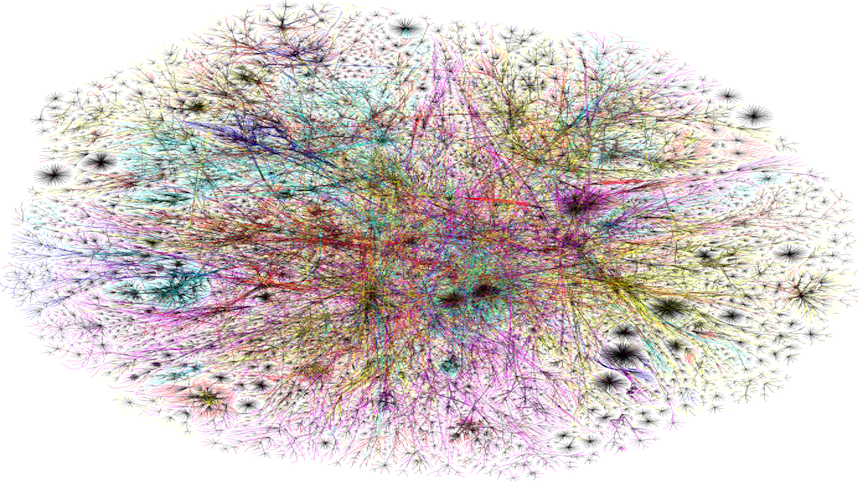
\includegraphics{opte.png}
\caption{Figure from opte.}
\label{fig:opte}
\end{center}
\end{figure}

This work has an explicit focus on \emph{paths} being a very essential property of networks.

